%You can leave alone everything before Line 79.
\documentclass{article}
\usepackage{url,amsfonts, amsmath, amssymb, amsthm,color, enumerate}
% Page layout
\setlength{\textheight}{8.75in}
\setlength{\columnsep}{2.0pc}
\setlength{\textwidth}{6.5in}
\setlength{\topmargin}{0in}
\setlength{\headheight}{0.0in}
\setlength{\headsep}{0.0in}
\setlength{\oddsidemargin}{0in}
\setlength{\evensidemargin}{0in}
\setlength{\parindent}{1pc}
\newcommand{\shortbar}{\begin{center}\rule{5ex}{0.1pt}\end{center}}
%\renewcommand{\baselinestretch}{1.1}
% Macros for course info
\newcommand{\courseNumber}{ME 552}
\newcommand{\courseTitle}{Mechatronics}
\newcommand{\semester}{Fall 2012}
\newcommand{\xxx}[1]{\textcolor{red}{#1}}
% Theorem-like structures are numbered within SECTION units
\theoremstyle{plain}
\newtheorem{theorem}{Theorem}[section]
\newtheorem{lemma}[theorem]{Lemma}
\newtheorem{corollary}[theorem]{Corollary}
\newtheorem{proposition}[theorem]{Proposition}
\newtheorem{statement}[theorem]{Statement}
\newtheorem{conjecture}[theorem]{Conjecture}
\newtheorem{fact}{Fact}
%definition style
\theoremstyle{definition}
\newtheorem{definition}[theorem]{Definition}
\newtheorem{example}{Example}
\newtheorem{problem}[theorem]{Problem}
\newtheorem{exercise}{Exercise}
\newtheorem{algorithm}{Algorithm}
%remark style
\theoremstyle{remark}
\newtheorem{remark}[theorem]{Remark}
\newtheorem{reduction}[theorem]{Reduction}
%\newtheorem{question}[theorem]{Question}
\newtheorem{question}{Question}
%\newtheorem{claim}[theorem]{Claim}
%
% Proof-making commands and environments
\newcommand{\beginproof}{\medskip\noindent{\bf Proof.~}}
\newcommand{\beginproofof}[1]{\medskip\noindent{\bf Proof of #1.~}}
\newcommand{\finishproof}{\hspace{0.2ex}\rule{1ex}{1ex}}
\def\therefore{\boldsymbol{\text{ }
\leavevmode
\lower0.4ex\hbox{$\cdot$}
\kern-.5em\raise0.7ex\hbox{$\cdot$}
\kern-0.55em\lower0.4ex\hbox{$\cdot$}
\thinspace\text{ }}}

\newenvironment{solution}[1]{\medskip\noindent{\bf Problem #1.~}}{\shortbar}

%====header======
\newcommand{\solutions}[4]{
%\renewcommand{\thetheorem}{{#2}.\arabic{theorem}}
\vspace{-2ex}
\begin{center}
{\small  \courseNumber, \courseTitle
\hfill {\Large \bf {#1} }\\
\semester, University of Michigan, Ann Arbor \hfill
{\em Date: #3}}\\
\vspace{-1ex}
\hrulefill\\
\vspace{4ex}
{\LARGE Lab Assignment #2}\\
\vspace{2ex}
\end{center}
\begin{trivlist}
\item \textsc{Team members:\\} {#4}
\end{trivlist}
\noindent
\shortbar
\vspace{3ex}
}
% math macros
\newcommand{\defeq}{\stackrel{\textrm{def}}{=}}
\newcommand{\Prob}{\textrm{Prob}}
%==
\usepackage{graphicx}
\begin{document}
%%%%%%%%%%%%%%%%%%%%%%%%%%%%%%%%%%%%%%%%%%%%%%%%%
%\solutions{Your name}{Problem Set Number}{Date of preparation}{Collaborators}{Prover}{Verifiers}
\solutions{}{2(A): MagLev}{\today}{Shiva Ghose, @gshiva\\ John Peterson, @jrpeters\\ Peter Turpel, @pturpel\\ Chan-Rong Lin, @pmelin}
%%%%%%%%%%%%%%%%%%%%%%%%%%%%%%%%%%%%%%%%%%%%%%%%%
%\renewcommand{\theproblem}{\arabic{problem}} 
%%%%%%%%%%%%%%%%%%%%%%%%%%%%%%%%%%%%%%%%%%%%%%%%%
%
% Begin the solution for each problem by
% \begin{solution}{Problem Number} and ends it with \end{solution}
%
% the solution for Problem 
\section*{Teamwork Participation Pledge :: Team 1}

I attest that I have made a fair and equitable contribution to this lab and submitted 
assignment. \\

My signature also indicates that I have followed the University of Michigan Honor Code, 
while working on this lab and assignment.\\

I accept my responsibility to look after all of the equipment assigned to me and my team, 
and that I have read and understood the X50 Lab Rules.\\

\begin{table}[h]
\begin{center}
    \begin{tabular}{|c|c|c|}
        \hline
        \textbf{Name} & \textbf{Email}     & \textbf{ \ \ \ \ \  \ \  \ \ \ \ \  \ \ Signature  \ \ \ \ \  \ \ \ \ \ \ \  \ \ } \\ \hline
        	~& ~& ~\\
	~& ~& ~\\
	Shiva Ghose   & gshiva@umich.edu   & ~                  \\
	~& ~& ~\\
	~& ~& ~\\ \hline 
	~& ~& ~\\
	~& ~& ~\\
        John Peterson & jrpeters@umich.edu & ~                  \\ 
	~& ~& ~\\
	~& ~& ~\\ \hline 
	~& ~& ~\\
	~& ~& ~\\
        Peter Turpel   & pturpel@umich.edu & ~                  \\
	~& ~& ~\\
	~& ~& ~\\ \hline 
	~& ~& ~\\
	~& ~& ~\\
        Chan-Rong Lin   & pmelin@umich.edu & ~                  \\
	~& ~& ~\\
	~& ~& ~\\ \hline 
        \hline
    \end{tabular}
\end{center}
\end{table}

\newpage


\section*{Part 1 Question 1}
\subsection*{a.}
The system can be represented as a block diagram as shown in figure \ref{q1_a1}. The individual subsystems can be seen in figure \ref{q1_a2}
\begin{figure}[h]
\begin{center}
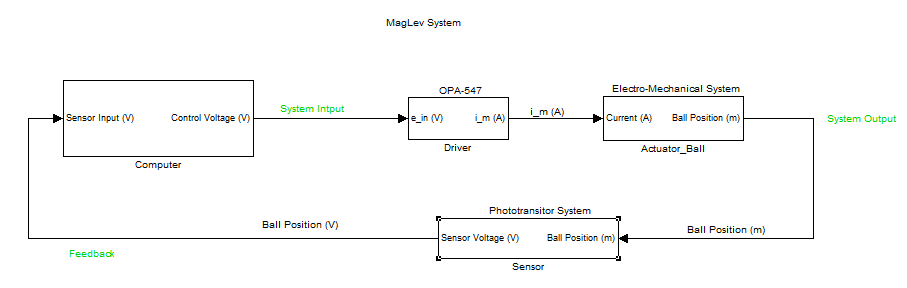
\includegraphics[width=10cm]{MagLevSystem.png}
\end{center}
\caption{Block diagram of the system.}
\label{q1_a1}
\end{figure}

Note that we used a non-linear matlab function to model the sensor system. The code is attached at the end of the report in the appendix.

\begin{figure}[h]
\begin{center}
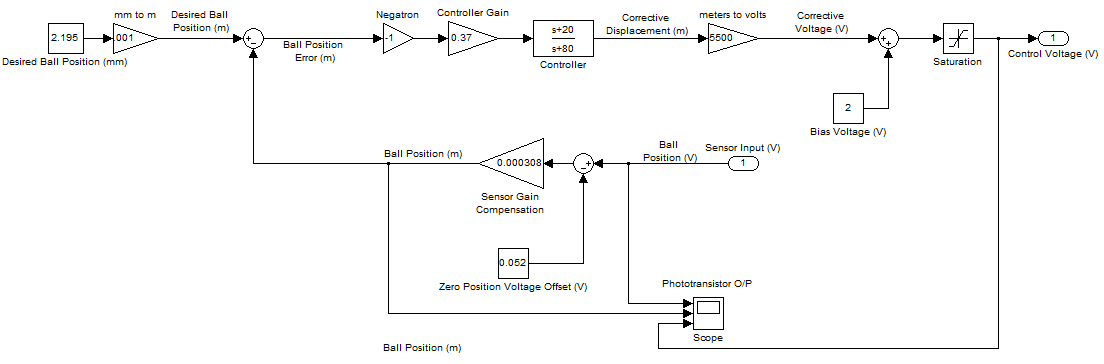
\includegraphics[width=15cm]{Computer.png}
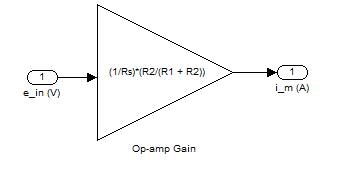
\includegraphics[width=5cm]{OpAmp.png}
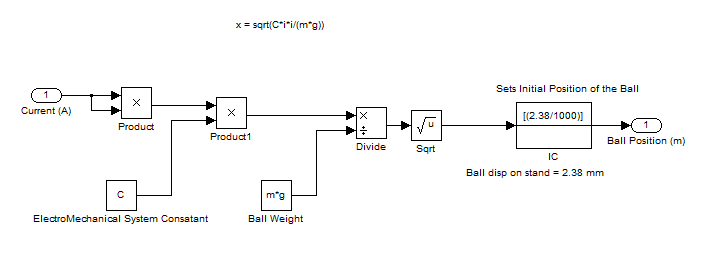
\includegraphics[width=10cm]{Actuator_Ball.png}
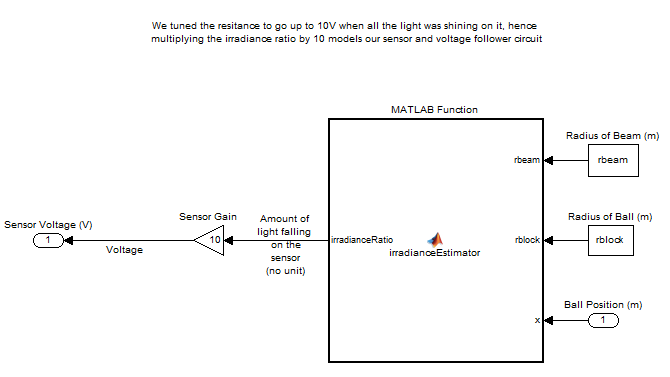
\includegraphics[width=8cm]{Sensor.png}
\end{center}
\caption{Block diagram of the sub-systems.}
\label{q1_a2}
\end{figure}


\subsection*{b.}
The bias voltage performs two functions in the circuit:
\begin{itemize}
\item The control system we have implemented operates on the change in position, $\hat{x}$, which is represented by a change in voltage ($\hat{V}$). However we would like the control be performed about a point of interest, $x_0$. The bias voltage holds the ball at $x_0$ at steady state in the absence of errors.

\item The second function of the bias voltage is to compensate for the steady state error in the system. The control system we have implemented is a Lead Compensator which minimizes the rate of change in error, $\Delta \emph{Error}$. However steady state errors are constant, $\Delta \emph{Error} = 0$. This can be compensated for using a Integral action or an offset-value.We chose to minimize the error using the bias voltage.
\end{itemize}

%The bias voltage helps compensate for the steady state errors in the system. In order to control the position of the ball, we have implemented a lead compensator. The differentiating action of the controller does not account for the steady state errors as the differential of a constant is zero. Thus we manually compensate for the constant errors using the bias voltage. The bias voltage accounts for the constant voltage required to support the weight of the sphere in steady state.  This bias voltage is necessary because because the controller operates on the difference of the measured position and the actual position.  We need this bias to reduce steady state error and generate a strong enough voltage command to the magnet.
\subsection*{c.}
The photo-transistor passes a current proportional to the amount of light falling on it.  However, our data acquisition card can only measure voltages, rather than currents, so we must convert this current signal into a voltage signal for the card to read by passing this current through a resistor (as seen in figure \ref{q1_c}). The resistance of this resistor has been adjusted to make use of the full input voltage range of the DAQ from 0 to 10 volts.\\ 

We require the voltage following amplifier to avoid loading the sensor circuit when we measure the voltage across this resistor.  This is not strictly necessary when using the DAQ because of its high input impedance ( greater than 10 $G\Omega$) but when we eventually physically implement our controller this may not be the case.  


\begin{figure}[h]
\begin{center}
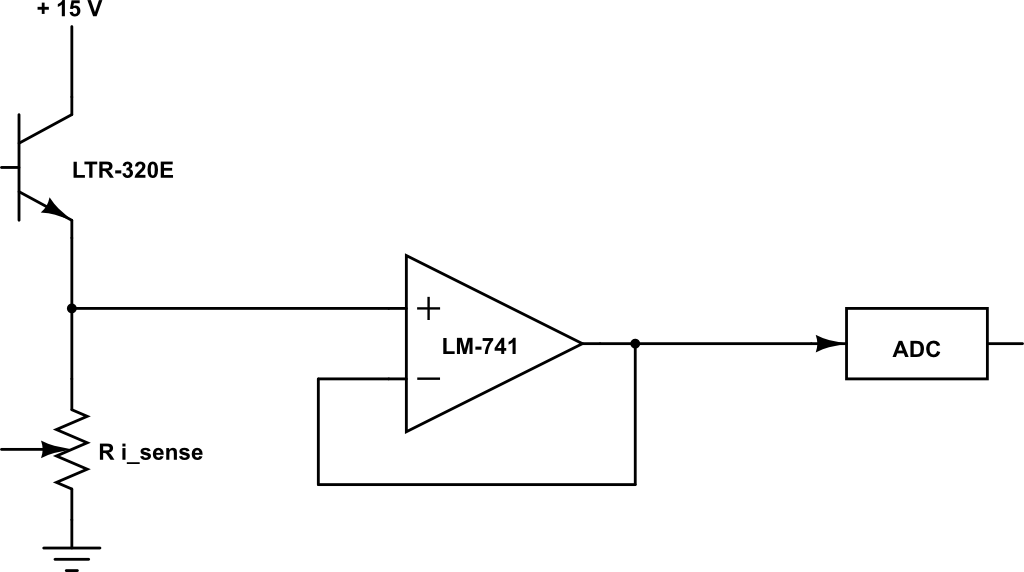
\includegraphics[width=8cm]{lab2_sensorckt.png}
\end{center}
\caption{Circuit diagram of the photo-detector setup.}
\label{q1_c}
\end{figure}


\subsection*{d.}
The minimum resistance that can be used in the emitter circuit is dictated by the maximum amount of current that the IR LED can draw, in steady state, without burning out.  

\begin{center}
$$ V_{LED}=1.6 \hspace{0.1cm} V \hspace{1cm} I_{max} = 0.2 \hspace{0.1cm} A $$ \\
$$ \Sigma{V} = V_{supply} - V_{LED} - V_0 = 15 - 1.6 - V_0 = 0 \hspace{1cm} V_0=13.4=IR $$\\
$$ V_0=I_{max}R_{min} \hspace{1cm} R_{min}=\frac{V_0}{I_{max}}=\frac{13.4 \hspace{0.1cm} V}{0.2 \hspace{0.1cm} A} = 67\hspace{0.1cm} \Omega$$\\
\end{center}

\begin{figure}[h]
\begin{center}
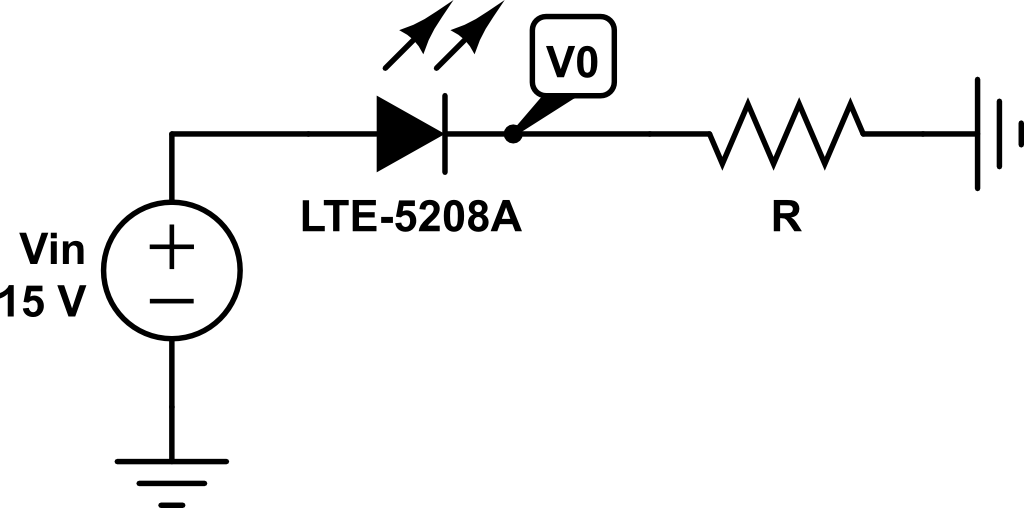
\includegraphics[width=10cm]{lab2_emitter.png}
\end{center}
\caption{Simplified lead-lag compensator circuit diagram.}
\label{q1_b}
\end{figure}

A lower resistance allows the circuit to pass more current resulting in a brighter IR beam. This brighter beam results in a higher signal to noise ratio, because this extra brightness will help to overpower ambient IR sources. It does not effect the full scale range of our detector circuit because this resistance has been tunned to ensure that range between the unblocked beam and the fully occluded beam is 10 volts.  \\  

\subsection*{e.}
It depends on the nature of the failure. 

\begin{itemize}
\item If $R_{Lim}$ fails by shorting out then the maximum current is 750 $mA$ \\

$$I_{Lim} = \frac{(5000)*(4.75)}{31600\Omega + R_{CL}} $$

\item If $R_{Lim}$ is intact and another component fails, then the maximum current is 510 $mA$. \\

$$I_{Lim} = \frac{(5000)*(4.75)}{31.600k\Omega + 14.9k\Omega} =510.64mA$$

\item If the electromagnet somehow became shorted across $+V$ and $-V$, then it would see a potential difference of 30 V.  The coil's internal resistance is 32 $\Omega$ yielding a current of 0.9375 A, and a power dissipated of 28.125 W, which may be enough to cause the coil to overheat.\\


$$I = \frac{V}{R} = \frac{30}{32} = 0.9375 A \hspace{1cm}  P = \frac{V^{2}}{R} = \frac{30^2}{32} = 28.125 W $$
\end{itemize}

If the coil shorted out but remained in series with any of the other components, most of them would be unable to handle the large current draw and rapidly fail.  We would recommend a fuse in series with the coil with 10\% more current rating than our current limit, yielding a rating of 560 $mA$\\


\subsection*{f.}  We would like the lower limit to be 0 volts, because feeding negative voltage to the magnet would elicit the non-linear behavior of the electromagnet.  In a linear system, we would expect this negative signal to push the sphere away, but in this non-linear system it would attract the sphere.  Limiting the lower range to 0 avoids this non-linearity.  
Our present current limit is 510 $mA$.  This current would require an input voltage of 12.07 $V$ into the driver circuit.  Our DAQ is limited to a maximum output of 10 V, and in practice even with the beam unobstructed the system demands approximately 2.5 V, but with transient effects will demand upwards of $55$ M$V$ if the sensor reading steps through its full scale, 0 to 10V range in a single time step. Making it necessary to limit the maximum command voltage to a sensible value.  We chose 5 volts as this does not seem to affect steady state operation and the limit is high enough to allow spikes in the control voltage that the controller wants.

$$V_{command} \approx P * \frac{dV_{sensor}}{dt}  = \frac{0.37 * 5500 * (10 - 0)}{0.001} = 5.5*10^7$$

%Since we are using this voltage to control current, we want to limit the voltage to limit the current to a safe level that can be maintained to not overheat the coil.

Additionally we would also like to avoid unnecessarily heating the coil with excessive current. As we control the current using voltage, limiting it to 5V additionally prevents heating stress on the coil.

\subsection*{g.}
No, the polarity of the electro-magnet does not matter in this application because either pole of the magnet will attract a piece of ferromagnetic material.  The expression for the force exerted by the magnet is given by:
$$\text{Force } = -C\Big(\frac{i}{x}\Big)^2$$

Where $C$ is the elctro-magnet's coefficient of attraction, $i$ is the current flowing through the circuit and $x$ is the vertical displacement of the ball from the electro-magnet. The negative sign indicates that the force is attractive in nature.\\

We see that the force is independent of the polarity of $i$ as it is proportional to $i^2$, which will always be positive.


\subsection*{h.}
The capacitors act as filters that remove high frequency noise in the power supply. They act similar to a fly-wheel in an engine where they maintain a constant voltage across their terminals, even in the presence of high frequency changes to the input.\\

The power supply provided in the X-50 lab is already buffered and smoothened out. Hence, when we removed the capacitors, the system did not show any noticeable change in behavior.

\section{Part 2 Question 1}

\subsection*{a.}

\subsubsection{Break Beam Sensor}

Assumptions \\
\begin{itemize}
\item Neglect Diffraction.
\item Light rays are parallel. 
\end{itemize}
As a consequence of these two assumptions the IR beam from the LED to the photo-transistor can be modeled as a cylinder.  The shadow casted by the sphere is then simply the circle with radius equal to the radius of the sphere.  This also means that the distance between the sphere and the IR LED does not matter, instead the only values that matter are the radius of the IR beam, the radius of the sphere, and the perpendicular distance between the axis of the beam and the center of the sphere.  The amount of light received by the photo-transistor can then simply be modeled as the intersection of two circles in 2-dimensions. \\

%\begin{algorithm}
%\IF{r_{beam} + \abs{d} < r_{sphere}
%\ENDIF
%\end{algorithm}

 %\begin{center}
%$$Power Fraction = PF = \frac{A_{beam} - A_{blocked}}{A_{beam}} $$ \\

%\end{center}

\subsubsection{Electro Magnet}

\subsubsection{Bearing \& Magnet System}

\subsection*{b.}

\subsection*{c.}

\subsection*{d.}

\subsection*{e.}

\subsection*{f.}

\subsection*{g.}

\section{Part 2 Question 2}

\subsection*{a.}

\subsection*{b.}

\subsection*{c.}

\subsection*{d.}

\section{Part 2 question 3}
%These capacitors buffer the large current requirements of the electromagnet when it turns on. 
%$V_i(t) = L\frac{di(t)}{dt}$
%
%\xxx{need picture of nominal response with and without capacitors should see difference}\\
%\xxx{graph of supply voltages and see if lack of capacitor is messing them up}\\
%
%\xxx{make note of our use of the flyback diode, want to show that it improves response, so run an experiment and compare transient current response with and without it in place} \\
%
%\xxx{make a note of vdroop on sensor} \\
\newpage
\section*{Appendix}
\subsection*{irradianceEstimate.m}
\begin{verbatim}
function [irradianceRatio] = irradianceEstimate(rbeam, rblock, x)
% computes the fraction of irradiance as a function of the radii of the two
% intersecting circles and the distance between their centers, d
% This can be used to model the irradiance of our phototransistor if we
% make several assumptions:
% - ignore diffraction
% - assume parallel light rays from LED to photo transistor so that we can
% model the * note we should use the minimum radius of the LED and the
% phototransistor - since - the parallel ray assumption means that distance
% from the ball to the LED doesn't matter

% let r1 be the beam radius and r2 be the blocking radius

% details at http://mathworld.wolfram.com/Circle-CircleIntersection.html

% estimated rblock = 6.35 mm
% estimated rbeam as = 2.3650 mm radius of the phototransistor

% regressed rbeam = 1.5048

assert((rbeam >= 0) && (rblock >= 0), 'The radii should be non-negative');

r1 = rbeam;
r2 = rblock;

d = x - 2.23;

if ((r1 > r2) && ((r2 + abs(d)) < r1))
    % handle the block is completely in the beam and the beam is bigger
    A1 = pi * r1 * r1;
    A2 = pi * r2 * r2;
    
    irradianceRatio = (A1 - A2) / A1;
    
elseif ((r2 >= r1) && ((r1 + abs(d)) <= r2))
    % handle case where block is larger or same size than beam and completely in the way
    irradianceRatio = 0;
        
elseif (abs(d) < (r1 + r2))
    % handle case where two circles intersect each other
    x = (d * d + r1 * r1 - r2 * r2) / (2 * d);
    
    d1 = x;
    d2 = (d * d - r1 * r1 + r2 * r2) / (2 * d);
    
    A = cSarea(r1, d1) + cSarea(r2, d2);
    
    Amax = pi * r1 * r1;
    
    irradianceRatio = (Amax - A) / Amax;

else 
    % handle case with no overlap
    irradianceRatio = 1;
end


irradianceRatio = irradianceRatio * 10;
end

function [area] = cSarea(r, h) 
% computes the area of the circular segment where the upper boundary is a
% circular arc and the lower boundary is a cord of the circle with radius r
% h is the perpendicular distance from the center to the cord

area = r * r * acos(h / r) - h * sqrt(r * r - h * h);

end
\end{verbatim}

\end{document}